\documentclass{beamer}

\usetheme[]{Rochester}
\usecolortheme{beaver}
\usepackage[latin1]{inputenc}
\usepackage{graphics}

\author{Will Webberley}
\date{Autumn 2014}
\institute[COMSC]{Cardiff School of Computer Science and Informatics}



\title{Heuristic evaluation}
\subtitle{CM2101: Human-Computer Interaction}

\begin{document}

\frame{\titlepage}

\frame{
    \frametitle{Revisiting Neilsen's heuristics}
    \begin{enumerate}
        \item Visibility of system status
        \begin{itemize}
            \item System should inform users about what's going on internally.
        \end{itemize}
        \item Match between system and real world
        \begin{itemize}
            \item System should speak the user's language and allow functions in a logical order.
        \end{itemize}
        \item User control and freedom
        \begin{itemize}
            \item Provide an `emergency exit' (e.g. by allowing an `undo' action)
        \end{itemize}
        \item Consistency and standards
        \begin{itemize}
            \item Ensure that different words or actions don't mean the same thing. Follow the platform guidelines.
        \end{itemize}
        \item Error prevention
        \begin{itemize}
            \item As well as using good error messages, try and prevent errors from happening.
        \end{itemize}
    \end{enumerate}
}

\frame{
    \frametitle{Revisiting Neilsen's heuristics}
    \begin{enumerate}
        \setcounter{enumi}{5}
        \item Recognition rather than recall
        \begin{itemize}
            \item Reduce users' memory loads by making actions and options visible. Use standard practices.
        \end{itemize}
        \item Flexibility and efficiency
        \begin{itemize}
            \item Cater to both expert and unexperienced users by making it faster to use for experts.
        \end{itemize}
        \item Aesthetic and minimalist design
        \begin{itemize}
            \item Do not display irrelevant information. Keep interface concise and provice contextually relevant actions.
        \end{itemize}
        \item Help users recognise, diagnose, and recover from errors
        \begin{itemize}
            \item Use English, avoid error codes, constructively provide a solution.
        \end{itemize}
        \item Help and documentation
        \begin{itemize}
            \item If you \textit{do} need documentation, make it easily searchable and task-focussed.
        \end{itemize}
    \end{enumerate}
}

\frame{
    \frametitle{Heuristic evaluation}
    \begin{itemize}
        \item Another type of evaluation (after user evaluation)
        \item Performed by an \alert{expert}
        \item Essentially, the UI is thoroughly inspected and \alert{usability problems are listed}
        \item \textit{Every} problem should be listed
        \item May need to go through twice (allowing a time to get the hang of the system)
        \item The Heuristics (e.g. Neilsen's) are used for \alert{justifying} the problems
    \end{itemize}
}

\frame{
    \frametitle{Heuristic evaluation: small example}
    \centering
    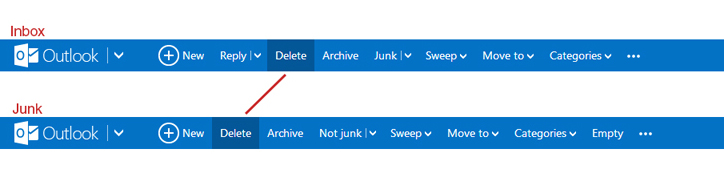
\includegraphics[width=11cm]{media/outlook.jpg}    
    \vskip20pt
    Same actions in different places in very similar views. This violates \alert{consistency} and \alert{recognition \& recall}.
}

\frame{
    \frametitle{}}

\end{document}
